
\chapter{Design of foot sensors pressure acquisition} % (fold)
\label{appendix:design_FSR}


\section{Principles} % (fold)
To obtain measurement of the pressure variation under our Poppy's feet we used FSR sensors from Interlink Electronics (see \figurename~\ref{fig:FSR_explode_view}). The FSR sensor will vary its resistance depending on how much pressure is being applied to the sensing area. The harder the force, the lower the resistance is. These sensors are low-cost -6\$ each- yet theirs behaviors are very non-linear (see \figurename~\ref{fig:foot_sensor_behavior}) and the calibration is quite variable depending on the production batch and the thermal conditions. So we cannot expect having precise results.

\begin{figure}[h]
\centering
    \subfloat[][Exploded view\footnote{Illustration credit: \url{http://www.openmusiclabs.com/learning/sensors/fsr/}} of a FSR sensor]{\label{fig:FSR_explode_view}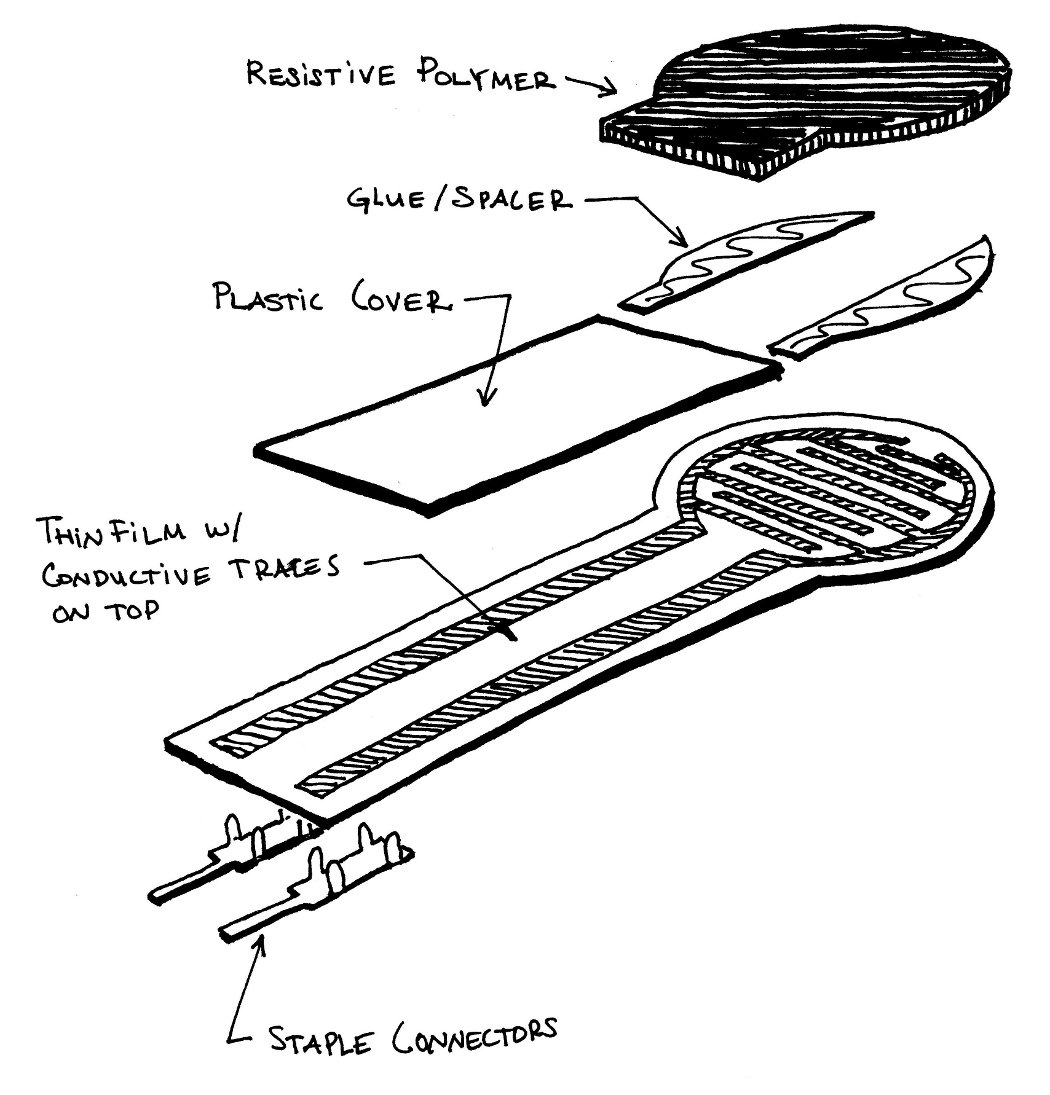
\includegraphics[height=6.3cm]{FSR_explode_view.jpg}}
    \hfil
    \subfloat[][Measured FSR sensor resistance depending on the applied force.]{\label{fig:FSR_behavior}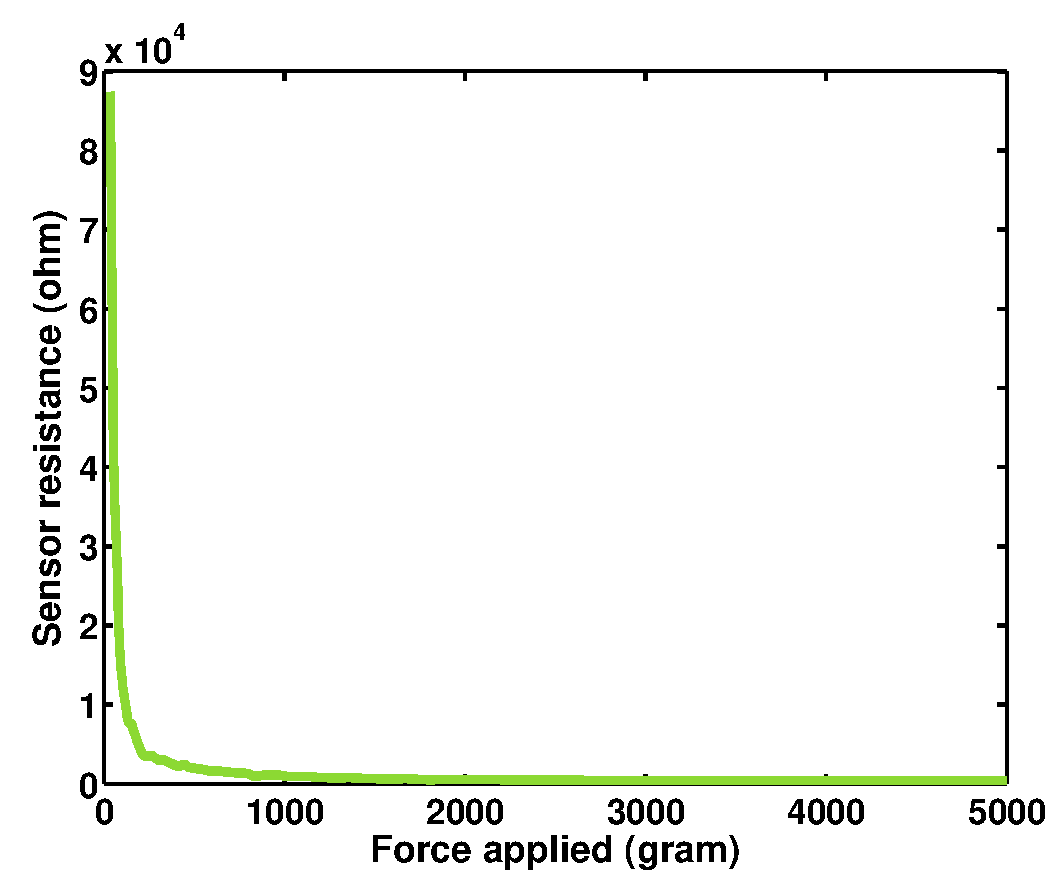
\includegraphics[height=6.3cm]{FSR_behavior.pdf}}
    \caption{The FSR force sensors are cheap but they have a really non-linear behavior and are not very precise.}
    \label{fig:}
\end{figure}

The acquisition of the resistance can be done indirectly by designing a voltage-divider\footnote{A voltage divider is a linear circuit that produces an output voltage $V_{out}$ that is a fraction of its input voltage $V_{in}$. It often consists of 2 resistors in series.} and using the FSR resistance variations to make the voltage output varies (see \equationname~\ref{eq:voltage-divider}). This voltage ($V_{out}$) can be then measured by an analog input of an Arduino board (see \figurename~\ref{fig:foot_sensors_test}).

\begin{equation}
    V_\mathrm{out} = \frac{R}{R+R_\mathrm{FSR}} \cdot V_\mathrm{in}
\label{eq:voltage-divider}
\end{equation}


\begin{figure}[!h]
\centering
    \subfloat[][A FSR sensor connected with Arduino nano board.]{\label{fig:foot_sensors_test}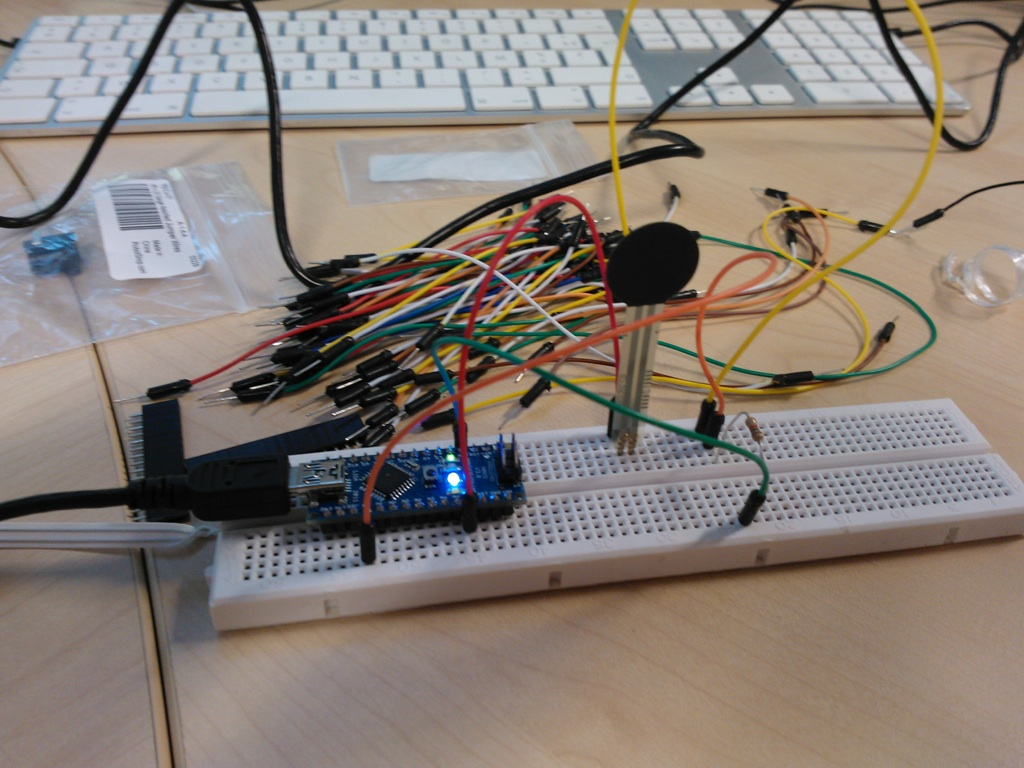
\includegraphics[height=5cm]{force_sensors_test.jpg}}
    \hfil
    \subfloat[][Simple testing assembly with 4 voltage dividers with FSR sensors and potentiometers plugged on an Arduino nano board]{\label{fig:}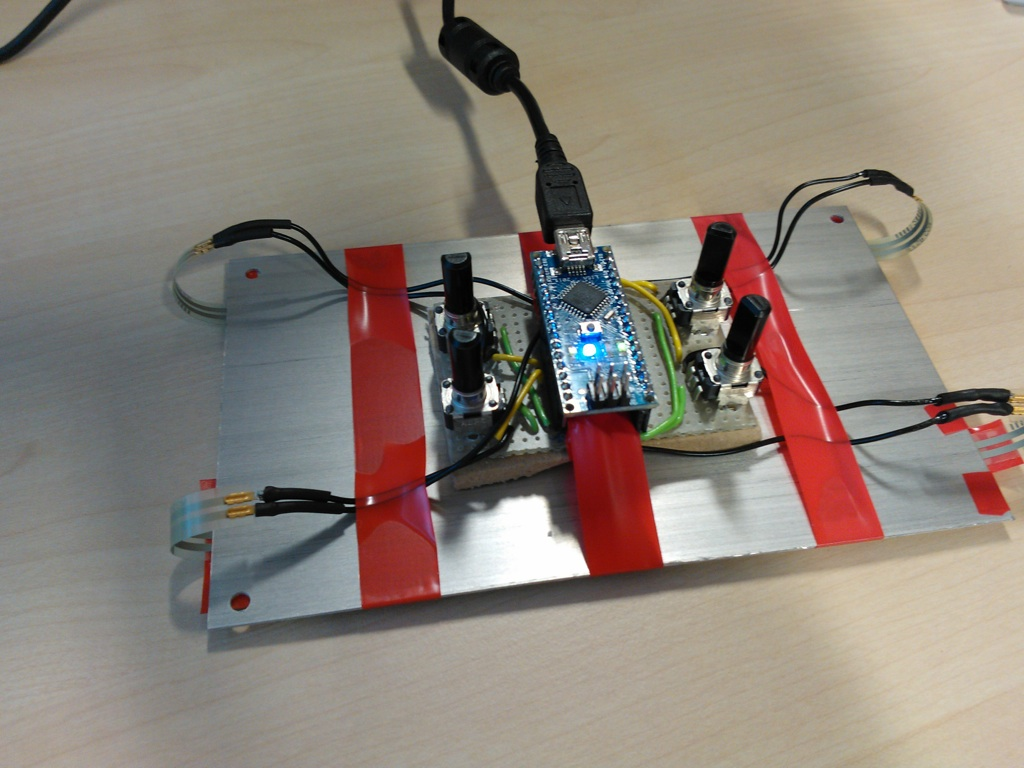
\includegraphics[height=5cm]{foot_sensors_proto.jpg}}
    \caption{We can easily measure the resistance variation of a FSR sensor using a voltage divider with the $V_{out}$ connected to an Arduino analog port.}
    \label{fig:test_sensors}
\end{figure}

\section{Design of the voltage divider to reduce the sensor non-linearity} % (fold)

A well tuned voltage-divider can help to reduce the non-linearity of the FSR sensors. Thus we conducted an optimization on the constant resistor choice depending on:
\begin{itemize}
    \item the Arduino analog precision: $1024$ values for a $5V$ input range,
    \item the use of the Dynamixel tension as voltage input i.e. $14V$,
    \item the standard resistor E12 precision series,
\end{itemize}

With an objective function sets to minimize the difference between the actual voltage-divider behavior and the perfect linear behavior $V_\mathrm{out}(F) = \alpha \cdot F$ with $V_\mathrm{out}(3.5kg) = 5V$ (see red curve on \figurename~\ref{fig:obtained_FSR_behavior}), we obtained the choice of a $180\Omega$ resistor for the constant resistance of the voltage divider (see \figurename~\ref{fig:FSR_best_resistor}). The best behavior found is plotted in blue on the \figurename~\ref{fig:obtained_FSR_behavior}.

\begin{figure}[h]
\centering
    \subfloat[][Optimization of the voltage divider constant resistor: distance between the output behavior with respect to a linear behavior.]{\label{fig:FSR_best_resistor}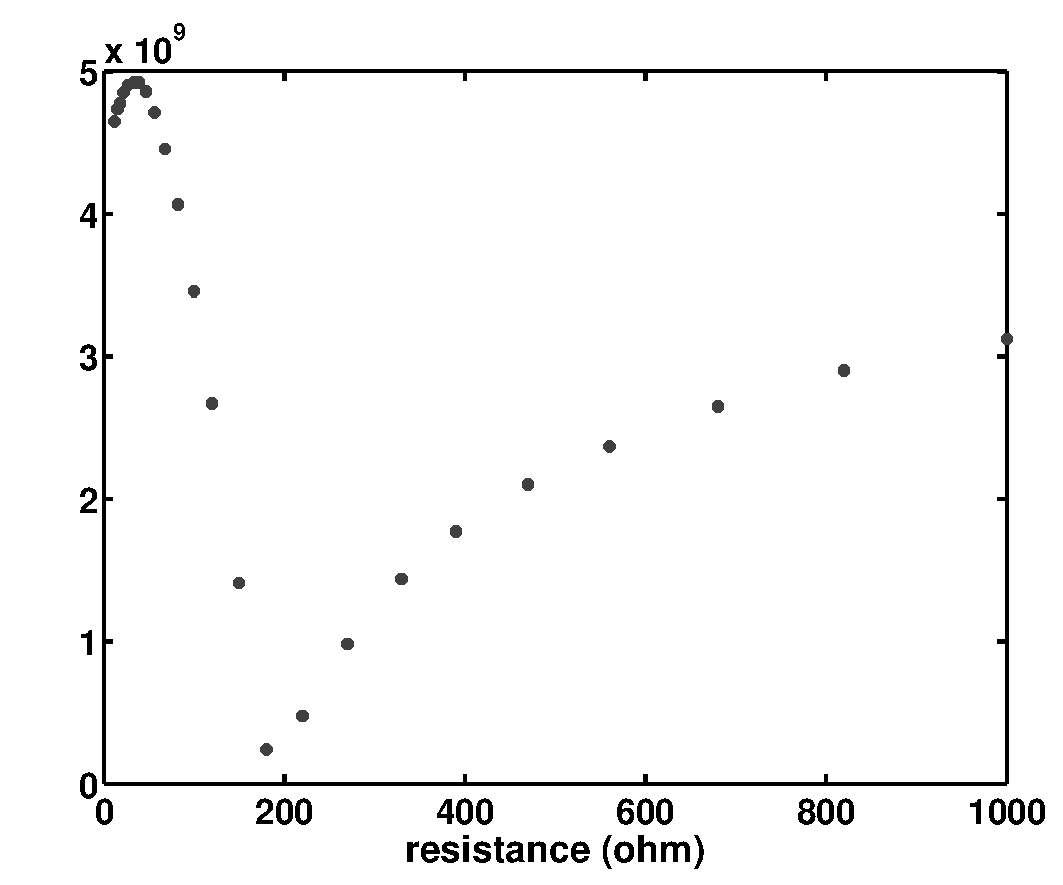
\includegraphics[width=0.48\linewidth]{criteria_dist.pdf}}
    \hfil
    \subfloat[][Theoretical behavior (blue) of the output voltage with respect to the applied force with a $14v$ input and a $180\Omega$ compared with the objective linear behavior.]{\label{fig:obtained_FSR_behavior}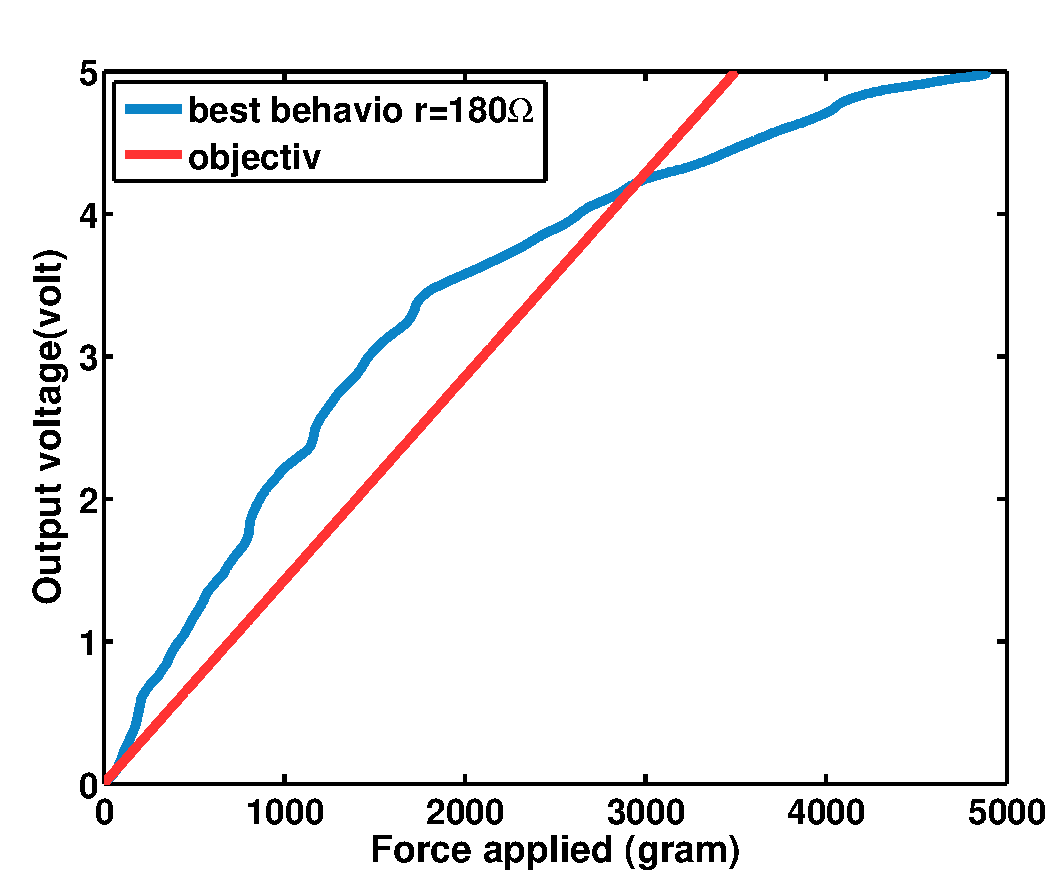
\includegraphics[width=0.48\linewidth]{voltage_behavior.pdf}}
    \caption{The design of the voltage divider for each FSR sensor is done by optimizing the output behavior toward a ideal linear behavior.}
    \label{fig:foot_sensor_behavior}
\end{figure}
